\documentclass{article}
\usepackage{natbib}
\usepackage{natbib,letltxmacro}
 \usepackage{float}
\usepackage{lineno}

% Language setting
% Replace `english' with e.g. `spanish' to change the document language
\usepackage[english]{babel}

% Set page size and margins
% Replace `letterpaper' with `a4paper' for UK/EU standard size
\usepackage[letterpaper,top=2cm,bottom=2cm,left=3cm,right=3cm,marginparwidth=1.75cm]{geometry}

% Useful packages
\usepackage{amsmath}
\usepackage{graphicx}
\usepackage[colorlinks=true, allcolors=blue]{hyperref}

\title{Predictive Identification of Tyrosinase Bacteria\\
using Machine Learning}
\author{Mingji Zhang (mz522@imperial.ac.uk)\\\\
Supervised by :\\
Samraat Pawer ( Imperial College London)}
\date{Apr,2023}
\footnotetext[2]{CMEECoursework,Department of Life Sciences, Imperial College of Science, Technology and Medicine}

\begin{document}

\maketitle
\newpage

\section{background}
 Lysine decarboxylase is an enzyme that catalyzes the hydrolysis of lysine, breaking it down into substrate and amino acid\citep{panis2021expression}. It plays an important role in ecological environments, such as participating in nitrogen cycling. Lysine decarboxylase catalyzes the decomposition of lysine to produce amino acids, including glutamate and aspartate, which can enter the nitrogen cycle and supply the nitrogen element needed for organisms to synthesize proteins and other nitrogenous compounds\citep{panis2021expression,}. Lysine decarboxylase also participates in bacterial metabolism, helping some bacteria metabolize or degrade lysine compounds from within or outside the organism. In addition, lysine decarboxylase is associated with photosynthesis in the ecosystem\citep{panis2022novel}. In some plants and plankton, lysine can participate in photosynthesis with chlorophyll and play an important role in the process.\\\\
The gene sequence of lysine decarboxylase is closely related to microorganisms. As the enzyme is encoded by genes, differences in the gene sequence of lysine decarboxylase may exist among different microorganisms. These differences may lead to variations in the catalytic activity, efficiency, thermal stability, and acid-alkali resistance of lysine decarboxylase in different microorganisms\citep{janusz2017lignin}.\\\\
Furthermore, differences in gene sequence may also result in certain microorganisms having special environmental adaptability, such as tolerance to high or low temperatures. These unique adaptabilities may give these microorganisms a competitive advantage in specific environments, thereby affecting the structure and function of the ecosystem\citep{panis2022novel}.\\\\
Therefore, studying the gene sequences of lysine decarboxylase in different microorganisms can provide valuable information to better understand their functions and adaptabilities, and to deepen our understanding of the role of microorganisms in the ecosystem.

\section{Method}
In recent years, machine learning has made significant progress and has been widely used in various fields, including bioinformatics .With the increase in big data and computing power, machine learning has become more efficient, accurate, and flexible, and has achieved great success in applications such as genome sequence analysis, protein structure prediction, and drug discovery\citep{moradigaravand2018prediction}.\\\\
The aim of this study is to explore the application of machine learning in genome sequence analysis and prediction, specifically in predicting bacteria containing TYR genes. To achieve this, various machine learning techniques will be employed, including Random Forest, deep learning algorithms and convolutional neural networks(Maybe). The raw genomic sequence data will be pre-processed to improve data quality and reliability, and performance evaluation metrics such as ROC curves, precision, and recall will be used to assess the model's effectiveness.\\\\
The expected outcome of this study is the development of an efficient and accurate prediction model for identifying bacteria containing TYR genes in large-scale genomic sequence data. This research will provide new methods and ideas for life science research, as well as advance the application of machine learning in bioinformatics\citep{moradigaravand2018prediction}..\\\\
In conclusion, machine learning has experienced significant development in recent years, and has proven to be highly effective in various fields, including bioinformatics. This study aims to further explore the application of machine learning in genome sequence analysis and prediction, and will employ various techniques to develop an accurate and efficient prediction model for identifying bacteria containing TYR genes. The results of this research will contribute to the advancement of bioinformatics and provide new insights into life science research.\\

\section{Work Steps}

1. Data Collection and Pre-processing\\\\
   The first step of this study involves collecting bacterial genome sequence data containing TYR genes from relevant databases. Subsequently, the collected data will undergo pre-processing, which includes gene assembly, redundancy removal, noise removal and error correction, in order to enhance data quality and reliability.\\\\
2. Feature Extraction and Data Cleaning\\\\
   Known features related to TYR genes will be extracted from the literature research of existing research results and utilized as known features to screen the bacterial genome sequence data. Furthermore, the filtered data will be cleaned to eliminate missing values and abnormal values to ensure data reliability.\\\\
3. Model Construction and Training\\\\
   The study will employ a random forest model for the classification and prediction of screened bacterial genome sequence data containing TYR genes. Random forest is an integrated learning-based classification model known for its high accuracy and generalisation performance. The model construction process will use known features for training, with model optimisation and tuning via cross-validation methods to enhance the accuracy and stability of the model.
4. Model Evaluation and Result Analysis\\\\
   Various evaluation metrics such as accuracy, recall, F1 value, and ROC curve will be employed to evaluate the performance of the constructed random forest model. Additionally, the classification prediction results will be analysed and interpreted to explore the biological significance and role of TYR genes in bacteria. Comparisons with other commonly used classification models will also be conducted.\\\\
5. Conclusion and Outlook\\\\
   This study aims to explore the feasibility of using machine learning models for predicting bacteria containing TYR genes and demonstrate the effectiveness of random forest models for this task. The study's outcomes are anticipated to offer novel insights and methods for bacterial classification and gene function prediction, further advancing the application of machine learning in the field of bioinformatics. In the future, the study's data volume can be expanded, and additional features and deep learning models introduced to enhance the accuracy and reliability of classification prediction.\\\\

\section{Timeline}

\begin{figure}
    \begin{center}
\centering
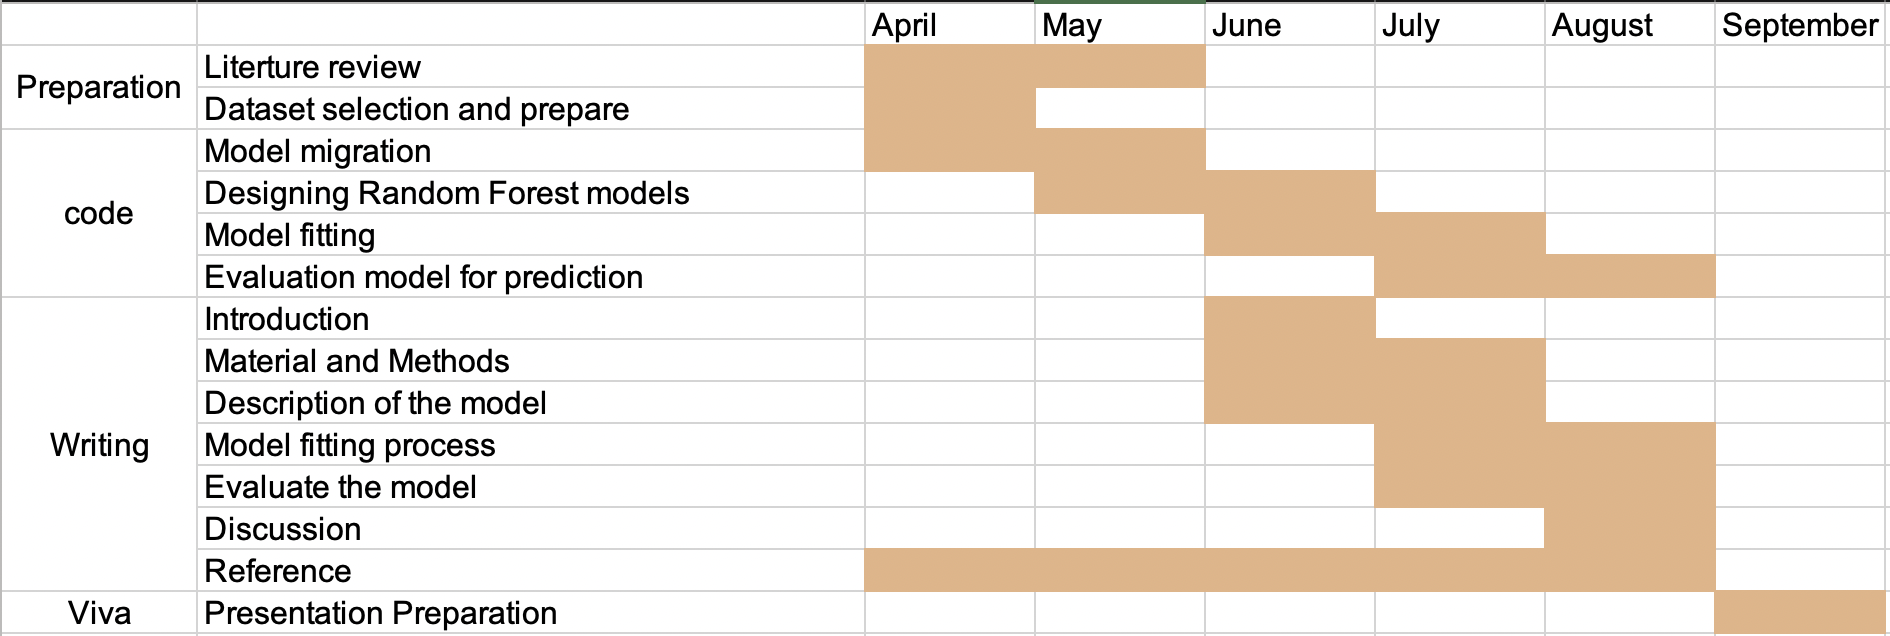
\includegraphics[scale= 0.5]{timeline.png}
\end{center}
\end{figure}

\newpage    
\bibliographystyle{apalike}
    \bibliography{proposalref}
\end{document}